%
% File acl2019.tex
%
%% Based on the style files for ACL 2018, NAACL 2018/19, which were
%% Based on the style files for ACL-2015, with some improvements
%%  taken from the NAACL-2016 style
%% Based on the style files for ACL-2014, which were, in turn,
%% based on ACL-2013, ACL-2012, ACL-2011, ACL-2010, ACL-IJCNLP-2009,
%% EACL-2009, IJCNLP-2008...
%% Based on the style files for EACL 2006 by 
%%e.agirre@ehu.es or Sergi.Balari@uab.es
%% and that of ACL 08 by Joakim Nivre and Noah Smith

\documentclass[11pt,a4paper]{article}
\usepackage[hyperref]{report}
\usepackage{times}
\usepackage{latexsym}
\usepackage{graphicx}
\graphicspath{{../figures/}}
\usepackage{url}

\aclfinalcopy % Uncomment this line for the final submission
%\def\aclpaperid{***} %  Enter the acl Paper ID here

%\setlength\titlebox{5cm}
% You can expand the titlebox if you need extra space
% to show all the authors. Please do not make the titlebox
% smaller than 5cm (the original size); we will check this
% in the camera-ready version and ask you to change it back.

\newcommand\BibTeX{B\textsc{ib}\TeX}

\title{Gendered Pronoun Resolution}

\author{Dhruv Patel \\
  IISc, Bangalore \\
  \texttt{dhruvpatel@iisc} \\\And
  Pratik Sachan \\
  IISc, Bangalore \\
  \texttt{pratiksachan@iisc} \\}

\date{}

\begin{document}
\maketitle
\begin{abstract}
  Abstract here.
\end{abstract}

\section{Datasets and Metrics}

\subsection{Datasets}

We have used two datasets in our experiments.
\begin{enumerate}
\item \textbf{GAP} GAP coreference dataset\cite{webster2018gap} is gender-balanced dataset devided into three sets for development, test and validation. Both development and test sets contain 2000 senteces each. Validation dataset contains 454 sentences. In each sentence there are two possible candidates denoted by A and B respectively. There is one pronoun per sentence. This pronoun can refer to either A or B or neither. Below is an example sentence from dataset. Bold italic is a pronoun. Bold words are candidate pronouns. Underlined noun is correct pronoun.
  \begin{quote}
    \textbf{\underline{Kathleen}} first appears when \textbf{Theresa} visits \textbf{\textit{her}} in a prison in London.
  \end{quote}

\item \textbf{DPR} Definite Pronoun Resolution \cite{rahman2012resolving} dataset is divided into two sets for traning and testing. There are 1886 sentences in total. Although the original dataset has only one candidate per sentence, there are two sentences having same actors in common(i.e. there are 943 pairs of senteces). So we combined two actors to play as candidates. The resulting dataset is similar to GAP. Below is an example pair.
  \begin{quote}
    \begin{itemize}
    \item James asked \textbf{Robert} for a favor, but \textit{\textbf{he}} refused.
    \item \textbf{James} asked Robert for a favor, but \textit{\textbf{he}} was refused.
    \end{itemize}
  \end{quote}
\end{enumerate}

We have used 2000 sentences from GAP to train, while keeping others aside for validation and test. When we used DPR in addition to GPR, we used both train and test sets for training. Validation in this case was still done on GAP validation set.

\subsection{Data Augmentation}

Earlier we tried our models without any data augmentation. But since GAP has only 2000 sentences in development set, our models overfitted. An SVM trained on these 2000 sentences outperformed neural network architectures that we tried. To compare our later modifications, we will use SVM as a baseline.

To mitigate the situation we applied data augmentation. Our hypothesis is that, since input to our network is just a pair of candidate nouns, it doesn’t matter what these nouns are. If all occurrences of noun `Firstname Lastname’ were to be replaced by some other plausible pair of first name and last names, sentence should make perfect sense. To neural network ``Jon Snow doesn’t know anything.’’ should be similar to ``John Wick doesn’t know anything.’’ 

To augment data we applied simple rule. If both candidate A and candidate B had less than four words then with probability 0.7 we would pick random noun with same number of words. That is if A had three words and B had two words, we would pick alternative A and B with three words and two words respectively. If pronoun is male then only male names are proposed as alternatives. Alternative name for B was chosen such that no word of it was a substring of alternative A. Also none of the alternatives had any overlap with original nouns. Below are the examples of augmented sentences. First sentence is an original, other are augmented. Here Margaret Ray is candidate A and Betsy is candidate B.

\begin{itemize}
\item Tony Markham, a high school senior and the ``Tall Dark Stranger'' \underline{Betsy} fell in love with as a freshman, who has since become a good friend not only to \underline{Betsy} but the entire \underline{Ray} family. \underline{Mrs. Ray}, \underline{Betsy}'s mother. \underline{Mr. Ray}, \underline{Betsy}'s father, who owns a shoestore. \textbf{\underline{Margaret Ray}}, \textbf{\underline{Betsy}}'s sister who is five years younger than she is.
  
\item Tony Markham, a high school senior and the ``Tall Dark Stranger'' \underline{Booth} fell in love with as a freshman, who has since become a good friend not only to \underline{Booth} but the entire \underline{Delgado} family. \underline{Mrs. Delgado}, \underline{Booth}'s mother. \underline{Mr. Delgado}, \underline{Booth}'s father, who owns a shoestore. \underline{Pam Delgado}, \underline{Booth}'s sister who is five years younger than she is.

\item Tony Markham, a high school senior and the ``Tall Dark Stranger'' \underline{Alyssa} fell in love with as a freshman, who has since become a good friend not only to \underline{Alyssa} but the entire \underline{Jolie} family. \underline{Mrs. Jolie}, \underline{Alyssa}'s mother. \underline{Mr. Jolie}, \underline{Alyssa}'s father, who owns a shoestore. \underline{Angelina Jolie}, \underline{Alyssa}'s sister who is five years younger than she is.
\end{itemize}

  
  The pool for alternative names was extracted from dataset for stage2 of Kaggle compitition. It has around 12K sentences. Figure \ref{fig:augment_dist} shows, distribution of names for both genders. One word names are most common in dataset followed by two word names.

  \begin{figure}
    \centering
    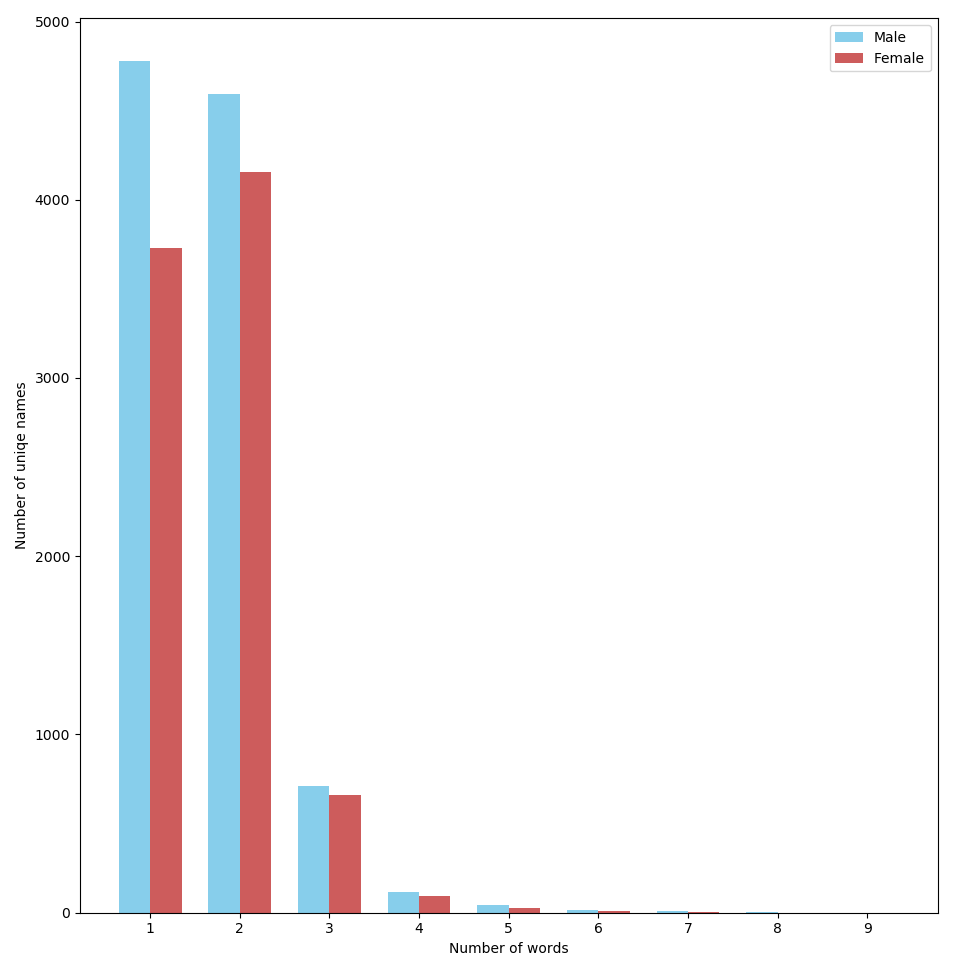
\includegraphics[width=.5\textwidth]{augment_dist.png}
    \caption{Distribution of names.}
    \label{fig:augment_dist}
  \end{figure}
  
  
\bibliography{report}
\bibliographystyle{acl_natbib}

\appendix

\end{document}
